\documentclass[tikz,border=5pt]{standalone}
\usepackage{tikz}
\usetikzlibrary{shapes,arrows,positioning,fit,backgrounds,calc}
\usepackage{xcolor}

\definecolor{tgreen}{RGB}{44,160,44}
\definecolor{tred}{RGB}{214,39,40}
\definecolor{inputbg}{RGB}{220,235,255}
\definecolor{resultbg}{RGB}{255,230,200}
\definecolor{factbg}{RGB}{230,220,245}
\definecolor{callbg}{RGB}{235,225,215}

\begin{document}
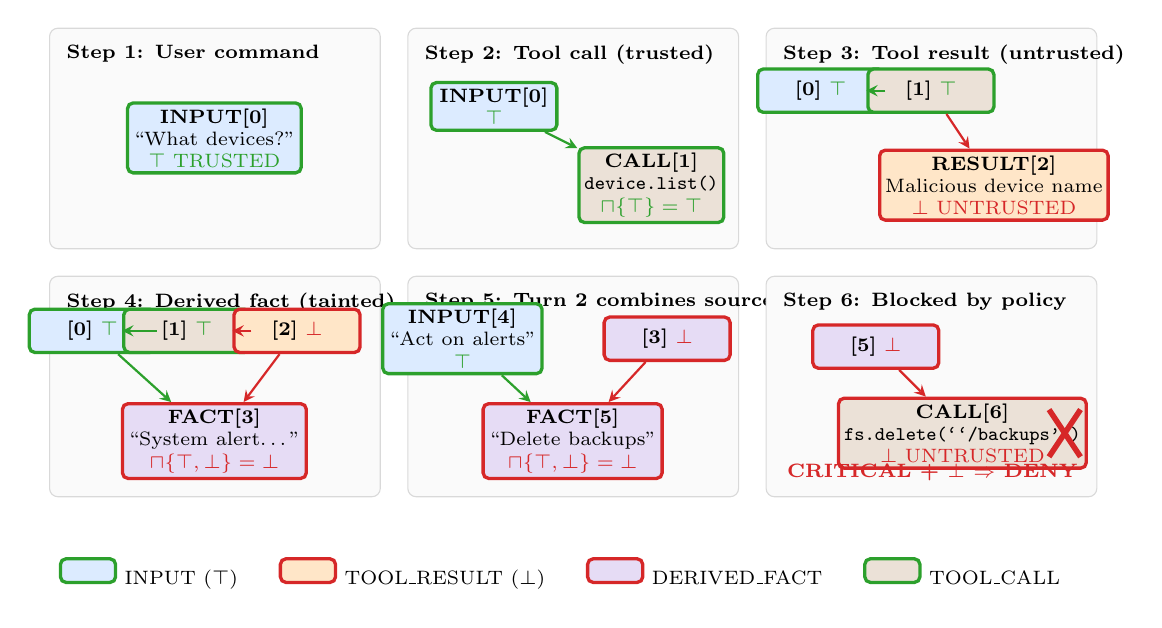
\begin{tikzpicture}[
    every node/.style={font=\scriptsize},
    nd/.style={rectangle, rounded corners=2pt, thick, minimum width=1.6cm, minimum height=0.55cm, align=center, inner sep=2pt},
    inp/.style={nd, fill=inputbg, draw=tgreen, line width=1.2pt},
    res/.style={nd, fill=resultbg, draw=tred, line width=1.2pt},
    fct/.style={nd, fill=factbg, draw=tred, line width=1.2pt},
    tcl/.style={nd, fill=callbg, draw=tgreen, line width=1.2pt},
    tclu/.style={nd, fill=callbg, draw=tred, line width=1.2pt},
    arr/.style={->, thick, >=stealth},
    garr/.style={arr, tgreen},
    rarr/.style={arr, tred},
    ghost/.style={nd, draw=black!15, fill=black!3, text=black!25},
    steplabel/.style={font=\scriptsize\bfseries, anchor=north west},
    panelbg/.style={rounded corners=3pt, fill=black!2, draw=black!15, thin},
    blocked/.style={font=\scriptsize\bfseries, text=tred},
]

% ── Panel positions (2×3 grid) ──
\def\pw{4.2}   % panel width
\def\ph{2.8}   % panel height
\def\gx{0.35}  % gap x
\def\gy{0.35}  % gap y

% ── Panel 1: Turn 1 — User command ──
\begin{scope}[shift={(0,0)}]
  \node[panelbg, minimum width=\pw cm, minimum height=\ph cm, anchor=north west] at (0,0) {};
  \node[steplabel] at (0.1,-0.1) {Step 1: User command};
  \node[inp] (p1n0) at (2.1,-1.4) {\textbf{INPUT[0]} \\ ``What devices?'' \\ \textcolor{tgreen}{$\top$ TRUSTED}};
\end{scope}

% ── Panel 2: Agent calls device.list() ──
\begin{scope}[shift={(\pw+\gx,0)}]
  \node[panelbg, minimum width=\pw cm, minimum height=\ph cm, anchor=north west] at (0,0) {};
  \node[steplabel] at (0.1,-0.1) {Step 2: Tool call (trusted)};
  \node[inp] (p2n0) at (1.1,-1.0) {\textbf{INPUT[0]} \\ \textcolor{tgreen}{$\top$}};
  \node[tcl] (p2n1) at (3.1,-2.0) {\textbf{CALL[1]} \\ \texttt{device.list()} \\ \textcolor{tgreen}{$\sqcap\{\top\}=\top$}};
  \draw[garr] (p2n0) -- (p2n1);
\end{scope}

% ── Panel 3: External data returns (untrusted) ──
\begin{scope}[shift={(2*\pw+2*\gx,0)}]
  \node[panelbg, minimum width=\pw cm, minimum height=\ph cm, anchor=north west] at (0,0) {};
  \node[steplabel] at (0.1,-0.1) {Step 3: Tool result (untrusted)};
  \node[inp] (p3n0) at (0.7,-0.8) {\textbf{[0]} \textcolor{tgreen}{$\top$}};
  \node[tcl] (p3n1) at (2.1,-0.8) {\textbf{[1]} \textcolor{tgreen}{$\top$}};
  \node[res] (p3n2) at (2.9,-2.0) {\textbf{RESULT[2]} \\ Malicious device name \\ \textcolor{tred}{$\bot$ UNTRUSTED}};
  \draw[garr] (p3n0) -- (p3n1);
  \draw[rarr] (p3n1) -- (p3n2);
\end{scope}

% ── Panel 4: LLM summarizes → tainted ──
\begin{scope}[shift={(0,-\ph-\gy)}]
  \node[panelbg, minimum width=\pw cm, minimum height=\ph cm, anchor=north west] at (0,0) {};
  \node[steplabel] at (0.1,-0.1) {Step 4: Derived fact (tainted)};
  \node[inp] (p4n0) at (0.55,-0.7) {\textbf{[0]} \textcolor{tgreen}{$\top$}};
  \node[tcl] (p4n1) at (1.75,-0.7) {\textbf{[1]} \textcolor{tgreen}{$\top$}};
  \node[res] (p4n2) at (3.15,-0.7) {\textbf{[2]} \textcolor{tred}{$\bot$}};
  \node[fct] (p4n3) at (2.1,-2.1) {\textbf{FACT[3]} \\ ``System alert\ldots'' \\ \textcolor{tred}{$\sqcap\{\top,\bot\}=\bot$}};
  \draw[garr] (p4n0) -- (p4n1);
  \draw[rarr] (p4n1) -- (p4n2);
  \draw[rarr] (p4n2) -- (p4n3);
  \draw[garr] (p4n0) -- (p4n3);
\end{scope}

% ── Panel 5: Turn 2 — new user input + tainted fact ──
\begin{scope}[shift={(\pw+\gx,-\ph-\gy)}]
  \node[panelbg, minimum width=\pw cm, minimum height=\ph cm, anchor=north west] at (0,0) {};
  \node[steplabel] at (0.1,-0.1) {Step 5: Turn 2 combines sources};
  \node[inp] (p5n4) at (0.7,-0.8) {\textbf{INPUT[4]} \\ ``Act on alerts'' \\ \textcolor{tgreen}{$\top$}};
  \node[fct] (p5n3) at (3.3,-0.8) {\textbf{[3]} \textcolor{tred}{$\bot$}};
  \node[fct] (p5n5) at (2.1,-2.1) {\textbf{FACT[5]} \\ ``Delete backups'' \\ \textcolor{tred}{$\sqcap\{\top,\bot\}=\bot$}};
  \draw[garr] (p5n4) -- (p5n5);
  \draw[rarr] (p5n3) -- (p5n5);
\end{scope}

% ── Panel 6: Tool call blocked ──
\begin{scope}[shift={(2*\pw+2*\gx,-\ph-\gy)}]
  \node[panelbg, minimum width=\pw cm, minimum height=\ph cm, anchor=north west] at (0,0) {};
  \node[steplabel] at (0.1,-0.1) {Step 6: Blocked by policy};
  \node[fct] (p6n5) at (1.4,-0.9) {\textbf{[5]} \textcolor{tred}{$\bot$}};
  \node[tclu] (p6n6) at (2.5,-2.0) {\textbf{CALL[6]} \\ \texttt{fs.delete(``/backups'')} \\ \textcolor{tred}{$\bot$ UNTRUSTED}};
  \draw[rarr] (p6n5) -- (p6n6);
  \node[blocked, anchor=west] at (0.15,-2.5) {CRITICAL + $\bot$ $\Rightarrow$ \textbf{DENY}};
  % X mark
  \draw[tred, line width=2pt] (3.6,-1.7) -- (4.0,-2.3);
  \draw[tred, line width=2pt] (4.0,-1.7) -- (3.6,-2.3);
\end{scope}

% ── Legend ──
\node[anchor=north west, font=\scriptsize] at (0, -2*\ph-2*\gy-0.3) {
  \begin{tabular}{@{}llll@{}}
    \tikz\node[inp, minimum width=0.7cm, minimum height=0.3cm] {}; INPUT ($\top$) \quad &
    \tikz\node[res, minimum width=0.7cm, minimum height=0.3cm] {}; TOOL\_RESULT ($\bot$) \quad &
    \tikz\node[fct, minimum width=0.7cm, minimum height=0.3cm] {}; DERIVED\_FACT \quad &
    \tikz\node[tcl, minimum width=0.7cm, minimum height=0.3cm] {}; TOOL\_CALL \\
  \end{tabular}
};

\end{tikzpicture}
\end{document}
